\PassOptionsToPackage{dvipsnames}{xcolor}
\documentclass{article}
\usepackage{graphicx,wrapfig,hyperref,pdfpages,geometry}

%for ALLOY
\usepackage[dvipsnames]{xcolor}
\usepackage{listings}
\usepackage{alloy-style}
\usepackage[T1]{fontenc}
\usepackage[utf8]{inputenc}

%substitute "{\em PowerEnJoy}" with "\pej"
\newcommand{\pej}{\mbox{\normalfont\itshape PowerEnJoy }}
%substitute "{\em CSGestion}" with "\csg"
\newcommand{\csg}{\mbox{\normalfont\itshape CSGestion }}
\newcommand{\version}{\mbox{\normalfont v. 1.1 }}

%to keep the links of the TOC invisible
\hypersetup{
	colorlinks,
	citecolor=black,
	filecolor=black,
	linkcolor=black,
	urlcolor=black
}

\geometry{margin=1in}



\begin{document}

	%---------------------------	FRONT PAGE      	-----------------------------
	\title{Politecnico di Milano\\A.A. 2016/2017\\Software Engineering 2: ``{\em PowerEnJoy}'' \version \\ \bigskip \textbf{R}equirements \textbf{A}nalysis and \textbf{S}pecification \textbf{D}ocument}
	\author{Matteo Bresich (mat. 774366)}
	
	
	%to avoid the hyphenation of the name
	\hyphenation{PowerEnJoy}
	
	\begin{figure}[t]
		\centering
		\includegraphics[width=\linewidth]{"img/logo-polimi"}
		\label{fig:polimi-logo}
	\end{figure}

	\maketitle
	
	%BLANK-PAGE
	\thispagestyle{empty}
	\clearpage\mbox{}\thispagestyle{empty}\clearpage
	
	\renewcommand*\thesection{\arabic{section}}
	\renewcommand*\thesubsection{\arabic{section}.\arabic{subsection}}
	\renewcommand*\thesubsubsection{%
		\arabic{section}.\arabic{subsection}.\arabic{subsubsection}%
	}
	\setcounter{secnumdepth}{4}
	\setcounter{tocdepth}{4}
	
	%---------------------------	TABLE OF CONTENT	-----------------------------
	%to change the page numbering from roman in the toc to arabic
	\pagenumbering{roman}
	\renewcommand{\contentsname}{Table of Content}
	\tableofcontents
	
	\newpage
	\pagenumbering{arabic}
	%to insert the writing "Page" above page numbers in the TOC
	\addtocontents{toc}{~\hfill\textrm{Page}\par}
	
	%---------------------------	INTRODUCTION		-----------------------------
	
	\section{Introduction}
	
		\subsection{Document Purpose}
		This document aims to describe in a complete way the application that will be developed and the domain in which it will be performed.\\
		The target audience of this document are analysts, project managers, developers, testers and final users.\\
		\textbf{Important!} This document has a contract validity between the costumer and the company that will develop the application.
		
		\subsection{Product Scope}
		\subsubsection{Actual system}
		Until now the car sharing company has a system where a registered client can reserve an electric car by calling a call-center. The service registration cannot be done on-line. It can only be done in the company office with a specific module. The company has a software called "\csg" that is a custom ERP, and it's used for managing all company cars. The software stores all the informations into a database.
		
		\begin{wrapfigure}{R}{0.35\textwidth}
			\centering
			\includegraphics[width=0.35\textwidth]{"img/eletronic-card"}
			\caption{\label{fig:eletronic-card} The electronic card obtained upon registration.}
		\end{wrapfigure}
		Data such as position, battery power and occupied seats are read by an on-board computer on every car and transmitted via cellular connection to the software. All data between the software \csg and each auto are transmitted using a VPN for better security on sensitive data.
		All customers requests are handled by the call-center of the company. An operator after a client request reserves the auto at most for one hour. The driver have to use an electronic card (
		obtained upon registration) for open the car. After the car is unlocked, the driver can turn on the machine by entering the user key (obtained upon registration) in the on-board computer and pushing the ignition button.
		When the driver leaves the car not in a safe area and gets out the car, can lock and unlock the car using the electronic card (Figure \ref{fig:eletronic-card}).
		After the use, when the driver gets out the car after leaving it in a safe area, the car will automatically lock.
		If the driver leaves the car in a safe area the payment of the service is automatically made by the registered client credit card and the car can be used by another customer.
		For whatever exception the client have to call the call-center.
		In case of accident it is provided that the car involved warns the system of the accident.
		A call-center operator will follow the practice and will notify to the company that deals with repairs.
		To ensure the proper functioning of the system the company hired employees (Handyman Operators) which in collaboration with the call-center recharges low battery cars and move cars from a safe area to another to ensure that in each area there is the minimum number of cars available.
			
		\subsubsection{Scope} \label{sec:scope}
		\pej is a new web and native mobile application thought to improve existing car sharing service. In particular \pej is focused to reduce unnecessary calls to the call-center, to facilitate the work of handyman operators, to simplify user ways to access to the service (for example using the smartphone to lock/unlock the booked car or provide an on-line registration) and advertise the car sharing service.
		\pagebreak
	
		\subsection{Definitions, acronyms, and abbreviations}
		\subsubsection{Definitions}
			\begin{itemize}
				\item Visitor (or Guest): is a non-registered user.
				\item User (or Registered User, or Client, or Driver): is the user of the application that wants to use the car sharing service.
				\item Passenger: is a person that use a car of the service that is not a driver. He/She has no obligation to be registered to the service.
				\item Location: are the GPS coordinates to identify a place. It could be the position of a car.
				\item Car (or Auto, or Transport): is a machine that belongs to the car sharing company.
				\item Safe area (or Equipped Parking): is a parking area defined in collaboration with the municipal administration equipped with charging towers for company cars. Every parking is unattended and for safety reasons equipped with CCTV.
				\item CSGestion: is an existing software used by call-center operators for managing all company cars. It allows to know for every car: car status (Available, Busy or Not working), the percentage of battery charge and the number of seats occupied.
				\item Lock/Unlock a car: it's means to lock/unlock the car door and deny/allow to a person to get in/out the car.
			\end{itemize}
		\subsubsection{Acronyms}
			\begin{itemize}
				\item RASD: Requirements Analysis and Specification Document.
				\item CSGestion: Car Sharing Gestion. 
				\item ERP: Enterprise Resource Planning.
				\item GPS: Global Positioning System.
				\item VPN: Virtual Private Network.
				\item CCTV: Closed Circuit Television.
			\end{itemize}
		\subsubsection{Abbreviations}
			\begin{itemize}
				\item App: application.
				\item {[}G$n${]}: $n$\textsuperscript{th} goal.
				\item {[}D$n${]}: $n$\textsuperscript{th} domain assumption.
				\item {[}R$n${]}: $n$\textsuperscript{th} functional requirement.
			\end{itemize}
		\subsection{Identifying Stakeholders}
		The main direct stakeholders of this project are the Municipality of Milan and the car sharing company that together have funded the renovation of the transport service. When the application will be on-line other stakeholders will be some company employees and final users that will provide a feedback of the new system.
		\subsection{Identifying Actors}
			\begin{itemize}
				\item Registered Users: are the final users of the car sharing service. Only they can book a car by calling the call-center or by using the web or mobile app, and use it.
				\item Passenger: is a registered user that can reserve a number of seats of a shared ride using the\\ \pej application.
				\item Handyman Operator: is a company employee that recharges low battery cars and move cars from a safe area to another to ensure that in each area there is the minimum number of cars available.
			\end{itemize}
		\subsection{Goals} \label{sec:goals}
		\newcommand{\gSystemDiscounts}{{[}G1{]} The System has to encourage the user to have a good behaviour using discounts.}
\newcommand{\gSystemFees}{{[}G2{]} The System has to discourage the user to have a bad behaviour using fees.}
\newcommand{\gSystemDistribution}{{[}G3{]} The System has to ensure a good distribution of cars in the territory.}
\newcommand{\gSystemShare}{{[}G4{]} The System has to provide the ability to share a ride.}
\newcommand{\gVisitorSignUp}{{[}G5{]} The Visitor shall be able to sign-up via app.}
\newcommand{\gRegisteredLogin}{{[}G6{]} The Registered User shall be able to log into the service.}
\newcommand{\gRegisteredReserve}{{[}G7{]} The Registered User shall be able to reserve a car up to one hour before via app.}
\newcommand{\gRegisteredDeleteReservation}{{[}G8{]} The Registered User shall be able to remove a reservation before the reservation time runs out.}
\newcommand{\gRegisteredSearchDistance}{{[}G9{]} The Registered User shall be able to find the locations of available cars within a certain distance from him.}
\newcommand{\gRegisteredSearchAddress}{{[}G10{]} The Registered User shall be able to find the locations of available cars from a specified address.}
\newcommand{\gRegisteredLockUnlock}{{[}G11{]} The Registered User shall open/close a reserved car via app when he/she is close to it.}
\newcommand{\gPassengerShare}{{[}G12{]} The Passenger shall be able to use a car in shared mode.}
\newcommand{\gHandymanRecharge}{{[}G13{]} The Handyman Operator shall know the location of the car that has to be charged.}
\newcommand{\gHandymanReportIssue}{{[}G14{]} The Handyman Operator shall report any problem with a car.}
		
		\subsection{Proposed system}
		The new system will not replace the old one, it will be integrate with it. The proposed solution will be implemented in a client-server architecture and consists in a software composed by a website and a mobile application. Both parts communicate with a server which runs the business logic and accesses the DBMS. Both parts will be developed from scratch. The web version should be responsive for a better view on mobile devices. The native mobile version will be developed for iOS, Android and Windows Phone.
			
		\subsection{Reference Documents}
		\begin{itemize}
			\item ISO/IEC/IEEE 29148-2011 Systems and software engineering - Life cycle processes - Requirements engineering.
		\end{itemize}
	
		\subsection{Overview}
		\begin{itemize}
			\item Section 1: Introduction, provides a short description of the application to be realized.
			\item Section 2: Overall Description, focuses on features of the software, constraints and assumptions.
			\item Section 3: Specific Requirements, provides requirements, typical scenarios and use cases for a more easy to read of software functionalities.
		\end{itemize}
	\pagebreak
	
	%---------------------------	OVERALL DESCRIPTION	-----------------------------
	
	\section{Overall description}
	
		\subsection{Product perspective}
		\pej is a web and mobile application which is integrated with an other existing system. The application does provide some APIs for integration with future projects.
		\subsection{Product functions}
		The function summary can be taken directly from the section in the first part of this document {\em Scope} (see section~\ref{sec:scope}) and {\em Goals} (see section~\ref{sec:goals}).
		\subsection{Constraints}
		\subsubsection{Regulatory Policies \& Safety and security}
		The system must be in accordance with local laws and policies. It must ask the user for the permission to acquire, store and process personal data and web cookies. The system must offer the possibility to delete all personal data.
		\subsubsection{Hardware limitations}
		\pej requires a computer or a smartphone connected to the internet. The mobile app requires the GPS module. The following list highlights some minimal conditions under which the system must operate: 
		
			\begin{center}
				\begin{tabular}{ | l | p{5cm} |}
					\hline
					& Requirements for Mobile App\\ \hline
					Operating system & Android 4.4.2 or higher, iOS 9 or higher, Windows phone 8 or higher\\\hline
					CPU & dual-core @1.5Ghz\\\hline
					Memory & 1GB \\\hline
					Other & 3G connection @1,5 Mb/s \\\hline
				\end{tabular}
			\end{center}
			
			\begin{center}
				\begin{tabular}{ | l | p{5cm} |}
					\hline
					& Requirements for Web App\\ \hline
					Operating system & Windows, MacOS, Linux\\\hline
					CPU & single-core @3Ghz \\\hline
					Memory & 1GB \\\hline
					Other & 800x600 resolution \\\hline
				\end{tabular}
			\end{center}
		\subsubsection{Reliability requirements}
		The system must have a minimum availability of 98\%.
		\subsubsection{Criticality of the application} 
		The system is not used in critical applications for life.
		\subsubsection{Interfaces to other applications}
		\pej requires to access the Internet, requires Google Maps APIs to provide map visualizations
		and map-related services and requires \csg APIs for integrate the new application with the old system.
		\subsubsection{Parallel operation}
		\pej supports parallel operations from different users.
		\subsection{Assumptions}
		\begin{itemize}
			\item Cars available and bookable are always working.
			\item Bookable Cars are always connected to the company VPN.
			\item Every bookable Car always provides correct data such as: location, battery status and occupied seats.
			\item A car reservation can be cancelled by the user before start the ride.
			\item Payments are charged at the end of each ride.
			\item If the driver and all passenger get out the car and the car location is in a safe area the ride ended.
			\item Passengers can share a ride payments only if they are registered to the service.
			\item The division of payment between registered users is by weighted average to reserved seats.
			\item The old payment system can be changed for the addition of discounts and fees.
			\item The service is regarded as a metropolitan transport service. It is against the rules to get away for more than 30km from the city center.
			\item The company's employee is registered to the system at the time of hiring.
			\item After a ride, the user can connect the auto to the charging system, but it is not required.
			\item A user who has reserved a car and decided to share the ride have to wait all passengers who have reserved a seat at least until before that the reservation expires.
			\item The location of safe areas are known and recorded in the system.
			\item A registered user has only one active reservation at a time: he/she can reserve a car or a number of seats of a shared ride at a time.
		\end{itemize}

	
	
	%---------------------------	SPECIFIC REQUIREMENTS 	-----------------------------
	\section{Specific requirements}
		\subsection{External Interface Requirements} 
			\subsubsection{User Interfaces}
			Below there are some mock-ups of the user interface. Mock-ups are only for the main features of the system. The following is only a preview. It is not final and during development it is necessary to work closely with the customer.
			
			\pagebreak
			\paragraph{Registration} This page presents the registration form for the user.
			\begin{center}
				\includegraphics[width=0.6\linewidth]{"img/ui/registration"}
			\end{center}
			\pagebreak

			\paragraph{Login} This page presents the login form for the user.
			\begin{center}
				\includegraphics[width=0.6\linewidth]{"img/ui/login"}
			\end{center}
			\pagebreak
			
			\paragraph{Private Area} This page presents the private area for the registered user.
			\begin{center}
				\includegraphics[width=0.6\linewidth]{"img/ui/private-area"}
			\end{center}
			\pagebreak
			
			\paragraph{Private Employees Area} This page presents the private area for the Handyman Operator.
			\begin{center}
				\includegraphics[width=0.6\linewidth]{"img/ui/private-area-employee"}
			\end{center}
			\pagebreak
			
			\paragraph{Car Reservation Page} This page presents the car booking page for the registered user.
			\begin{center}
				\includegraphics[width=0.6\linewidth]{"img/ui/search-car"}
			\end{center}
			\pagebreak
			
			\paragraph{Reservation Management Page} Follows the managment reservation page for the registered user.
			\begin{center}
				\includegraphics[width=0.6\linewidth]{"img/ui/delete-reservation"}
			\end{center}
			\pagebreak
			
			\paragraph{Get Cars to Recharge Page} This page presents cars that have to be connect to the charging station for the Handyman Operator.
			\begin{center}
				\includegraphics[width=0.6\linewidth]{"img/ui/get-cars-recharge"}
			\end{center}
			\pagebreak
			
			\paragraph{Edit Profile} Follows the edit profile page for the registered user.
			\begin{center}
				\includegraphics[width=0.6\linewidth]{"img/ui/edit-profile"}
			\end{center}
			\pagebreak
		
			\subsubsection{Hardware Interfaces}
			\pej does not require additional Hardware interface.
			\subsubsection{Communication Interfaces}
			\pej uses the TCP transport protocol and HTTP/HTTP over SSL application layer protocol to guarantee the security of data transmission.
			
		\subsection{Functional Requirements}
		\subsubsection{\gSystemDiscounts}
\begin{itemize}
	\item {[}D1{]} The old payment system can be changed for adding discounts and fees.
	\item {[}D2{]} The cost of the service is calculated per hour (ex. 3,5h).
	\item {[}D3{]} The car provides occupied spots with weight sensors under seats.
	\item {[}R1{]} If the System detecs that the user tooks at least two other passengers onto the car for at least half of the trip (in time term when the machine is in motion), the system applies a discount of 10\% on the last ride.
\end{itemize}
\subsubsection{\gSystemFees}
\begin{itemize}
	\item {[}D1{]} The old payment system can be changed for adding discounts and fees.
	\item {[}D2{]} The old system has APIs to generate a payment.
	\item {[}D3{]} Access to APIs is provided only using the HTTPS protocol.
	\item {[}R1{]} If a car is not picked-up within one hour from the reservation the user pays a fee of 1 EUR.
\end{itemize}
\subsubsection{\gSystemDistribution}
\begin{itemize}
	\item {[}D1{]} The old system keeps track of the current cars' locations.
	\item {[}D2{]} The old system generate which cars has to be moved, the initial and the final location for the auto.
	\item {[}R1{]} The System has to generate a message to an Handyman Operator that contains: which car has to be moved, the initial and the final location for the auto.
\end{itemize}	
\subsubsection{\gSystemShare}
\begin{itemize}
	\item {[}D1{]} The old system keeps track of the current cars' locations.
	\item {[}D2{]} The old system has APIs to get available shared ride and to get for each ride available seats.
	\item {[}D3{]} Access to APIs is provided only using the HTTPS protocol.
	\item {[}R1{]} The System has to show a list of available shared ride.
	\item {[}R2{]} The System has to show ride details such as: initial location, final location, occupied seats.
\end{itemize}
\subsubsection{\gVisitorSignUp}
\begin{itemize}
	\item {[}D1{]} Phone number, email address and payments method for the registration are mandatory and must be valid.
	\item {[}R1{]} The User cannot register more than once.
	\item {[}R2{]} Unregistered users can only see information pages of the service, the sign up page and login page.
	\item {[}R3{]} The User must fill in all the mandatory fields, accept terms of use and the privacy policy of the service to successfully complete the registration process.
	\item {[}R4{]} If the User successfully complete the registration process the electronic card for unlock booked cars will be sent to the address of residence.
\end{itemize}
\subsubsection{\gRegisteredLogin}
\begin{itemize}
	\item {[}D1{]} Subscribers with the old system are already available in the database.
	\item {[}R1{]} If the Registered User hasn’t the correct login information cannot access the system.
	\item {[}R2{]} If the Registered User provides correct credentials the system will grant him/her the access.
\end{itemize}
\subsubsection{\gRegisteredReserve}
\begin{itemize}
	\item {[}R1{]} A car can be reserved by only one registered user at a time.
	\item {[}R2{]} A Registered User can choose if enable a shared ride or not.
	\item {[}R3{]} A Registered User can reserve only one car at time.
	\item {[}R4{]} A Registered User can reserve a car only if the last payment was done properly.
\end{itemize}
\subsubsection{\gRegisteredDeleteReservation}
\begin{itemize}
	\item {[}R1{]} The Registered User shall be able to remove a reservation before the reservation time runs out.
\end{itemize}
\subsubsection{\gRegisteredSearchDistance}
\begin{itemize}
	\item {[}D1{]} The GPS coordinates are always available and correct.
	\item {[}R1{]} The Registered User can search available cars that are no more than 4km distant from her/him simply providing his/her own position.
\end{itemize}
\subsubsection{\gRegisteredSearchAddress}
\begin{itemize}
	\item {[}D1{]} The GPS coordinates are always available and correct.
	\item {[}R1{]} The Registered User can search available cars that are no more than 4km distant from the address provided.
\end{itemize}
\subsubsection{\gRegisteredLockUnlock}
\begin{itemize}
	\item {[}D1{]} Every car can be locked and unlocked from the onboard computer.
	\item {[}D2{]} Every car has a bluetooth module connected to the onboard computer.
	\item {[}D3{]} The old system has APIs to locked and unlocked a selected car.
	\item {[}D4{]} Access to APIs is provided only using the HTTPS protocol.
	\item {[}R1{]} A Registered User can open and close a car previously reserved using the mobile app.
	\item {[}R2{]} A Registered User must to be close to the car not more than 5m.
	\item {[}R3{]} The Registered User's smartphone must have the application installed and the permissions for use the bluetooth.
\end{itemize}
\subsubsection{\gPassengerShare}
\begin{itemize}
	\item {[}R1{]} A Passenger can reserves a number of seats of a selected shared ride.
	\item {[}R2{]} A Passenger can make one reservation at a time.
	\item {[}R3{]} A Passenger after the booking must arrive at the place of departure before the estimated departure. The estimated departure is calculated from the difference between the car prenotation time and the current time.
\end{itemize}
\subsubsection{\gHandymanRecharge}
\begin{itemize}
	\item {[}D1{]} Every Handyman Operator has a business smartphone provided by the company with the app.
	\item {[}D2{]} The old system has APIs to get battery status for each available car.
	\item {[}D3{]} The old system has APIs to get a list of cars that have to be attach to the charging system.
	\item {[}D4{]} The old system keeps track of the current cars' locations.
	\item {[}R1{]} A Handyman Operator can get what are the cars that have to be attach to the charging system.
	\item {[}R2{]} A Handyman Operator can get where are the cars that have to be attach to the charging system.
\end{itemize}
\subsubsection{\gHandymanReportIssue}
\begin{itemize}
	\item {[}D1{]} Every Handyman Operator has a business smartphone provided by the company with the app.
	\item {[}R1{]} A Handyman Operator can send a report if there are any problem with cars.
\end{itemize}
		
		\pagebreak
		\subsection{Scenarios}
		\subsubsection{Scenario 1}
Chiara is an university student and a registered user to the service. Every day she uses public transportation to reach the school in the center of Milan. During the year because of the public transportation's strikes she is forced to find an alternative way to arrive at her destination.
Just the other week when she had to go to college for an exam, when she arrives to Cadorna station because of the metro service strike, decided to use the app \pej installed on her smartphone.
After checking that there is a car available in the equipped parking nearest her, she book it and went to the equipped parking to get to her destination. The car chosen is fully charged.
After using it for the most of the day Chiara brings back the car to the Cadorna's equipped parking. Once she parked, the system detects the end of the race and automatically computes the fare and applies a discount on this ride of 20\% because the battery car charge is more than 50\%. 
The transaction is performed automatically by the user's method of payment already chosen
\subsubsection{Scenario 2}
Antonio wants to spend the night at the club. He is registered to the car sharing service. He book a car by calling the call center. He gets the car at the equipped parking close to home by opening it with his smartphone, he goes to take Sofia and Elena. After a fun evening the group recovers the car to the disco's parking and return home. After bringing home all, Antonio brings the car to the initial equipped parking. Once he parked, the system detects the end of the race and automatically computes the fare and applies a discount on this ride of 10\% because for more than 50\% of the movement time, Antonio led at least two other passengers with him. The transaction is performed automatically by Antonio's method of payment already chosen
\subsubsection{Scenario 3}
Four friends live near Lambrate's station. They want to go to the San Siro stadium for a concert. Andrea is registered to the car sharing service. After checking that there is a car in Lambrate's station he goes to catch it. The group spent 30 minutes to arrive at the stadium. After the concert only Alessandro come back with Andrea. They spent 45 minutes because of an accident. At the end of the ride the system automatically computes the fare and doesn't apply a discount on this ride of 10\% because for more than 50\% of the movement time, there are only Andrea and Alessandro. The transaction is performed automatically by Andrea's method of payment already chosen
\subsection{Scenario 4}
Two group have to go from the Centrale's station to the Garibaldi's Station (both are equipped parking).
Adrian, Sonia and Alessandro are in the first group instead Claudio and Silvia are in the second group. Adrian and Claudio are registered to the service. Adrian reserves a car for a shared ride. Claudio looks for a shared ride and finds Adrian's ride and reserves the remaining two seats. When they arrive to Garibaldi's Station the ride is over and the system automatically computes the fare and applies a discount on this ride of 10\% because for more than 50\% of the movement time, the car was sold out.
The fare is shared between Adrian and Claudio (Adrian: 3/5 of the total amount, Claudio: 2/5 of the total amount). The transaction is performed automatically by the users' method of payment already chosen
\subsubsection{Scenario 5}
Alessia leaves the car at the Bovisa's equipped parking, despite the fact that the car needs to be recharged, she has no time to connect the car to the charging system. \\
Daniele, an handyman operator, using the \pej application is checking if there are cars that need to be recharged. The car number 5 needs to be connect. Daniele reach the car and connect it.
\subsubsection{Scenario 6}
Roberta, Maria and Luigi that have token their \pej's cars in other equipped parking leave them in the equipped parking A. The system realizes that there are too much cars in the equipped parking A and sends a message to  the handyman operator Fabio. The message says: "Move car 5 from the equipped parking A to the equipped parking B". Fabio moves the car to the indicated location.
		\pagebreak
		\subsection{UML Models}
		\subsubsection{Use Case}
		\begin{center}
			\includegraphics[width=0.9\linewidth]{"img/use-case-whole-system"}
		\end{center}
		\pagebreak
		
		\paragraph{Visitor registers to \pej}
			\begin{center}
				\begin{tabular}{| l | p{9cm} |}\hline
					Actor & Visitor\\\hline
					Goal & {[}G5{]} \\\hline
					Precondition & None\\\hline
					Event Flow & \begin{enumerate}
						\item Visitor on the home page clicks on "Register".
						\item Visitor fills all required fields.
						\item Visitor clicks on the "Send" button.
						\item The application saves data in the database.
					\end{enumerate}\\\hline
					Postcondition & Visitor completes the registration process, becomes a registered user and obtains the username and the password generated by the system through email. \\\hline
					Exceptions & {\begin{enumerate}
							\item The visitor is already a registered user.
							\item Data not valid or missing.
							\item The email chosen is already associated to another user.
						\end{enumerate} }\\\hline
					Exception Handling&All exceptions are handled alerting the visitor of the
					problem through an error message.\\\hline
				\end{tabular}
			\end{center}
		\pagebreak
		\begin{minipage}{\linewidth}
			\vspace*{-0.7cm}
			\makebox[\linewidth]{
				\includegraphics[keepaspectratio=true,scale=0.61]{"img/use-case-registration"}}
		\end{minipage}
		
		\vspace*{1cm}
		
		\noindent%
		\begin{minipage}{\linewidth}
			\vspace*{-0.7cm}
			\makebox[\linewidth]{
				\includegraphics[keepaspectratio=true,scale=0.59]{"img/sequence-diagram-registration"}}
		\end{minipage}
				
		\paragraph{Visitor login to \pej}
		\begin{center}
			\begin{tabular}{| l | p{9cm} |}\hline
				Actor & Visitor\\\hline
				Goal & {[}G6{]} \\\hline
				Precondition & The Visitor must be already registered.\\\hline
				Event Flow & \begin{enumerate}
					\item Visitor navigates to the login page.
					\item Visitor fills all required fields.
					\item Visitor clicks on the "Login" button.
				\end{enumerate}\\\hline
				Postcondition & The application verifies the credentials and if correct shows the home page for the registered user and promotes guest to registered user.\\\hline
				Exceptions & {\begin{enumerate}
						\item Data not valid or missing.
				\end{enumerate} }\\\hline
				Exception Handling&All exceptions are handled alerting the visitor of the
				problem through an error message.\\\hline
			\end{tabular}
		\end{center}
		\pagebreak
		\begin{minipage}{\linewidth}
			\vspace*{-0.7cm}
			\makebox[\linewidth]{
				\includegraphics[keepaspectratio=true,scale=0.70]{"img/use-case-login"}}
		\end{minipage}
		
		\vspace*{1cm}
		
		\noindent%
		\begin{minipage}{\linewidth}
			\vspace*{-0.7cm}
			\makebox[\linewidth]{
				\includegraphics[keepaspectratio=true,scale=0.67]{"img/sequence-diagram-login"}}
		\end{minipage}
	
		\pagebreak
		\paragraph{Registered User reserve a car using \pej}
		\begin{center}
			\begin{tabular}{| l | p{9cm} |}\hline
				Actor & Registered User\\\hline
				Goal & {[}G7{]} \\\hline
				Precondition & The Registered User must be already logged in.\\\hline
				Event Flow & \begin{enumerate}
					\item The Registered User search an available car within a certain distance from him or from a specified address.
					\item The Registered User selects the desired car from a list.
					\item The Registered User click on the "Reserve" button.
					\item The Registered User can choose if share his/her ride.
					\item The Registered User, in the case of shared ride, have to provide the arrival location and occupied seats.
				\end{enumerate}\\\hline
				Postcondition & The application reserve the selected car for one hour. A timer stars to check the hour when the reservation it's confirmed.\\\hline
				Exceptions & \begin{enumerate}
					\item Already reserved car
				\end{enumerate} \\\hline
				Exception Handling&All exceptions are handled alerting the Registered User of the
				problem through an error message.\\\hline
			\end{tabular}
		\end{center}
		\pagebreak
		\begin{minipage}{\linewidth}
			\vspace*{-0.7cm}
			\makebox[\linewidth]{
				\includegraphics[keepaspectratio=true,scale=0.70]{"img/use-case-add-reservation"}}
		\end{minipage}
		
		\vspace*{1cm}
		
		\noindent%
		\begin{minipage}{\linewidth}
			\vspace*{-0.7cm}
			\makebox[\linewidth]{
				\includegraphics[keepaspectratio=true,scale=0.675]{"img/sequence-diagram-add-reservation"}}
		\end{minipage}
		
		\pagebreak
		\paragraph{Registered User delete a reservation using \pej}
		\begin{center}
			\begin{tabular}{| l | p{9cm} |}\hline
				Actor & Registered User\\\hline
				Goal & {[}G8{]} \\\hline
				Precondition & The Registered User must be already logged in. The Registered User must have made a reservation. The reservation time is not exceeded.\\\hline
				Event Flow & \begin{enumerate}
					\item The Registered User select from the menu "Manage Active Reservation".
					\item The Registered User selects the unique active reservation.
					\item The Registered User click on the "Delete Reservation" button.
					\item The Registered User at the message "Are you sure?" clicks on the "Yes" button.
				\end{enumerate}\\\hline
				Postcondition & The application cancel reservation and changes the state of the car in available.\\\hline
				Exceptions & \begin{enumerate}
					\item Reservation is exceeded.
				\end{enumerate}\\\hline
				Exception Handling&All exceptions are handled alerting the Registered User of the
				problem through an error message.\\\hline
			\end{tabular}
		\end{center}
		\pagebreak
		\begin{minipage}{\linewidth}
			\vspace*{-0.7cm}
			\makebox[\linewidth]{
				\includegraphics[keepaspectratio=true,scale=0.70]{"img/use-case-del-reservation"}}
		\end{minipage}
		
		\vspace*{1cm}
		
		\noindent%
		\begin{minipage}{\linewidth}
			\vspace*{-0.7cm}
			\makebox[\linewidth]{
				\includegraphics[keepaspectratio=true,scale=0.68]{"img/sequence-diagram-del-reservation"}}
		\end{minipage}
		
		\pagebreak
		\paragraph{Registered User search available cars using \pej}
		\begin{center}
			\begin{tabular}{| l | p{9cm} |}\hline
				Actor & Registered User\\\hline
				Goal & {[}G9{]} \\\hline
				Precondition & The Registered User must be already logged in. The Registered User must provide his/her location.\\\hline
				Event Flow & \begin{enumerate}
					\item The Registered User select from the menu "Search Cars Near Me".
				\end{enumerate}\\\hline
				Postcondition & The application retrive all available cars near user location and show them in a list.\\\hline
				Exceptions & \begin{enumerate}
					\item No cars available.
				\end{enumerate}\\\hline
				Exception Handling&All exceptions are handled alerting the Registered User of the
				problem through an error message.\\\hline
			\end{tabular}
		\end{center}
		\begin{center}
			\begin{tabular}{| l | p{9cm} |}\hline
				Actor & Registered User\\\hline
				Goal & {[}G10{]} \\\hline
				Precondition & The Registered User must be already logged in. The Registered User must provide an address for the desidered start location.\\\hline
				Event Flow & \begin{enumerate}
					\item The Registered User select from the menu "Search Cars Near the Address".
				\end{enumerate}\\\hline
				Postcondition & The application retrive all available cars near the address provided and show them in a list.\\\hline
				Exceptions & \begin{enumerate}
					\item No cars available.
				\end{enumerate}\\\hline
				Exception Handling&All exceptions are handled alerting the Registered User of the
				problem through an error message.\\\hline
			\end{tabular}
		\end{center}
		\pagebreak
		\begin{minipage}{\linewidth}
			\vspace*{-0.7cm}
			\makebox[\linewidth]{
				\includegraphics[keepaspectratio=true,scale=0.75]{"img/use-case-search-cars"}}
		\end{minipage}
		
		\vspace*{1cm}
		
		\noindent%
		\begin{minipage}{\linewidth}
			\vspace*{-0.7cm}
			\makebox[\linewidth]{
				\includegraphics[keepaspectratio=true,scale=0.68]{"img/sequence-diagram-search-cars"}}
		\end{minipage}
		
		\pagebreak
		\paragraph{Registered User manage a reserved car using \pej}
		\begin{center}
			\begin{tabular}{| l | p{9cm} |}\hline
				Actor & Registered User\\\hline
				Goal & {[}G11{]} \\\hline
				Precondition & The Registered User must be already logged in. The Registered User must have made a car reservation. The car reservation is still active.\\\hline
				Event Flow & \begin{enumerate}
					\item The Registered User select from the menu "Manage Active Reservation".
					\item The Registered User click the "Open"/"Close" button.
				\end{enumerate}\\\hline
				Postcondition & The application unlock/lock the reserved car.\\\hline
				Exceptions & \begin{enumerate}
					\item Unable to open/close the car.
					\item The user is not close enough to the car
				\end{enumerate}\\\hline
				Exception Handling&All exceptions are handled alerting the Registered User of the
				problem through an error message.\\\hline
			\end{tabular}
		\end{center}
		\pagebreak
		\begin{minipage}{\linewidth}
			\vspace*{-0.7cm}
			\makebox[\linewidth]{
				\includegraphics[keepaspectratio=true,scale=0.73]{"img/use-case-manage-car"}}
		\end{minipage}
		
		\vspace*{1cm}
		
		\noindent%
		\begin{minipage}{\linewidth}
			\vspace*{-0.7cm}
			\makebox[\linewidth]{
				\includegraphics[keepaspectratio=true,scale=0.69]{"img/sequence-diagram-manage-car"}}
		\end{minipage}
		
		\pagebreak
		\paragraph{Passenger reserves a number of seats of a shared ride using \pej}
		\begin{center}
			\begin{tabular}{| l | p{9cm} |}\hline
				Actor & Passenger\\\hline
				Goal & {[}G12{]} \\\hline
				Precondition & The Passenger must be already logged in.\\\hline
				Event Flow & \begin{enumerate}
					\item The Passenger select from the menu "Join a Ride".
					\item The Passenger chooses at which shared ride he/she wish to join from a list.
					\item The Passenger must provide the number of the seats he/she wants to reserve.
				\end{enumerate}\\\hline
				Postcondition & The application reserves seats of the selected ride.\\\hline
				Exceptions & \begin{enumerate}
					\item Impossible to reserve seats.
					\item Wrong number of seats.
				\end{enumerate}\\\hline
				Exception Handling&All exceptions are handled alerting the Registered User of the
				problem through an error message.\\\hline
			\end{tabular}
		\end{center}
		\paragraph{Passenger delete a reservation of a shared ride using \pej}
		\begin{center}
			\begin{tabular}{| l | p{9cm} |}\hline
				Actor & Passenger\\\hline
				Goal & {[}G12{]} \\\hline
				Precondition & The Passenger must be already logged in.\\\hline
				Event Flow & \begin{enumerate}
					\item The Passenger selects from the menu "Manage Active Reservation".
					\item The Passenger selects the unique active reservation.
					\item The Passenger click on the "Delete Reservation" button.
					\item The Passenger at the message "Are you sure?" clicks on the "Yes" button.
				\end{enumerate}\\\hline
				Postcondition & The application delete the seats reservation.\\\hline
				Exceptions & \begin{enumerate}
					\item Reservation is exceeded.
				\end{enumerate}\\\hline
				Exception Handling&All exceptions are handled alerting the Registered User of the
				problem through an error message.\\\hline
			\end{tabular}
		\end{center}
		\pagebreak
		\begin{minipage}{\linewidth}
			\vspace*{-0.7cm}
			\makebox[\linewidth]{
				\includegraphics[keepaspectratio=true,scale=0.65]{"img/use-case-manage-passenger-reservation"}}
		\end{minipage}
		
		\vspace*{1cm}
		
		\noindent%
		\begin{minipage}{\linewidth}
			\vspace*{-0.7cm}
			\makebox[\linewidth]{
				\includegraphics[keepaspectratio=true,scale=0.74]{"img/sequence-diagram-passenger-add-reservation"}}
		\end{minipage}
	
		\pagebreak
		
		\noindent%
		\begin{minipage}{\linewidth}
			\vspace*{-0.7cm}
			\makebox[\linewidth]{
				\includegraphics[keepaspectratio=true,scale=0.74]{"img/sequence-diagram-passenger-del-reservation"}}
		\end{minipage}
	
		\pagebreak
		
		\paragraph{Handyman operator gets which and where are cars that have to be attach to the charging system using \pej}
		\begin{center}
			\begin{tabular}{| l | p{9cm} |}\hline
				Actor & Handyman operator\\\hline
				Goal & {[}G13{]} \\\hline
				Precondition & The Handyman operator must be already logged in.\\\hline
				Event Flow & \begin{enumerate}
					\item The Handyman operator selects from the menu "Get Cars to Recharge".
					\item The Handyman operator gets a car list order by distance from him/her.
					\item The Handyman operator click on the "More Info" button.
				\end{enumerate}\\\hline
				Postcondition & The application show which and where are available cars that have to be attach to the charging system. \\\hline
				Exceptions & \begin{enumerate}
					\item No cars to be recharged.
				\end{enumerate}\\\hline
				Exception Handling&All exceptions are handled alerting the Registered User of the
				problem through an error message.\\\hline
			\end{tabular}
		\end{center}
		\pagebreak
		\begin{minipage}{\linewidth}
			\vspace*{-0.7cm}
			\makebox[\linewidth]{
				\includegraphics[keepaspectratio=true,scale=0.66]{"img/use-case-recharge"}}
		\end{minipage}
		
		\vspace*{1cm}
		
		\noindent%
		\begin{minipage}{\linewidth}
			\vspace*{-0.7cm}
			\makebox[\linewidth]{
				\includegraphics[keepaspectratio=true,scale=0.63]{"img/sequence-diagram-recharge"}}
		\end{minipage}
	
		\pagebreak
		
		\paragraph{Handyman operator sends a report using \pej}
		\begin{center}
			\begin{tabular}{| l | p{9cm} |}\hline
				Actor & Handyman operator\\\hline
				Goal & {[}G14{]} \\\hline
				Precondition & The Handyman operator must be already logged in.\\\hline
				Event Flow & \begin{enumerate}
					\item The Handyman operator selects from the menu "Send a Report".
					\item The Handyman operator fills all required fields.
					\item The Handyman operator click on the "Send Report" button.
				\end{enumerate}\\\hline
				Postcondition & The application generate a report that is sent to the old system.  \\\hline
				Exceptions & \begin{enumerate}
					\item Data not valid or missing.
				\end{enumerate}\\\hline
				Exception Handling&All exceptions are handled alerting the Registered User of the
				problem through an error message.\\\hline
			\end{tabular}
		\end{center}
		\pagebreak
		\begin{minipage}{\linewidth}
			\vspace*{-0.7cm}
			\makebox[\linewidth]{
				\includegraphics[keepaspectratio=true,scale=0.70]{"img/use-case-report"}}
		\end{minipage}
		
		\vspace*{1cm}
		
		\noindent%
		\begin{minipage}{\linewidth}
			\vspace*{-0.7cm}
			\makebox[\linewidth]{
				\includegraphics[keepaspectratio=true,scale=0.62]{"img/sequence-diagram-report"}}
		\end{minipage}
		
		\pagebreak
		
		\subsubsection{Class Diagram}
		\begin{minipage}{\linewidth}
			\vspace*{1cm}
			\makebox[\linewidth]{
				\includegraphics[keepaspectratio=true,scale=0.40]{"img/class-diagram"}}
		\end{minipage}
		\pagebreak
		\subsubsection{State Machine Diagrams}
		
			\paragraph{Evolution of a Car Reservation} The following finite state machine shows the possible states of a car reservation and events that enable the change of state.\\
			\noindent%
			\begin{minipage}{\linewidth}
				%			\vspace*{-0.35cm}
				\makebox[\linewidth]{
					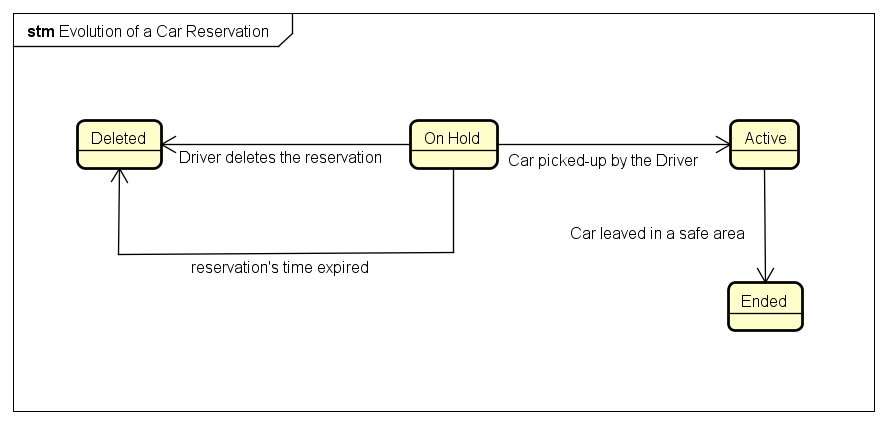
\includegraphics[keepaspectratio=true,scale=0.65]{img/state-machine-car-reservation}}
			\end{minipage}	
			
			\vspace*{1cm}
		
			\paragraph{Car Avaliability} The following finite state machine shows the possible
			states of Availability of a car and events that enable the change of state.\\
			\noindent%
			\begin{minipage}{\linewidth}
				%			\vspace*{-0.35cm}
				\makebox[\linewidth]{
					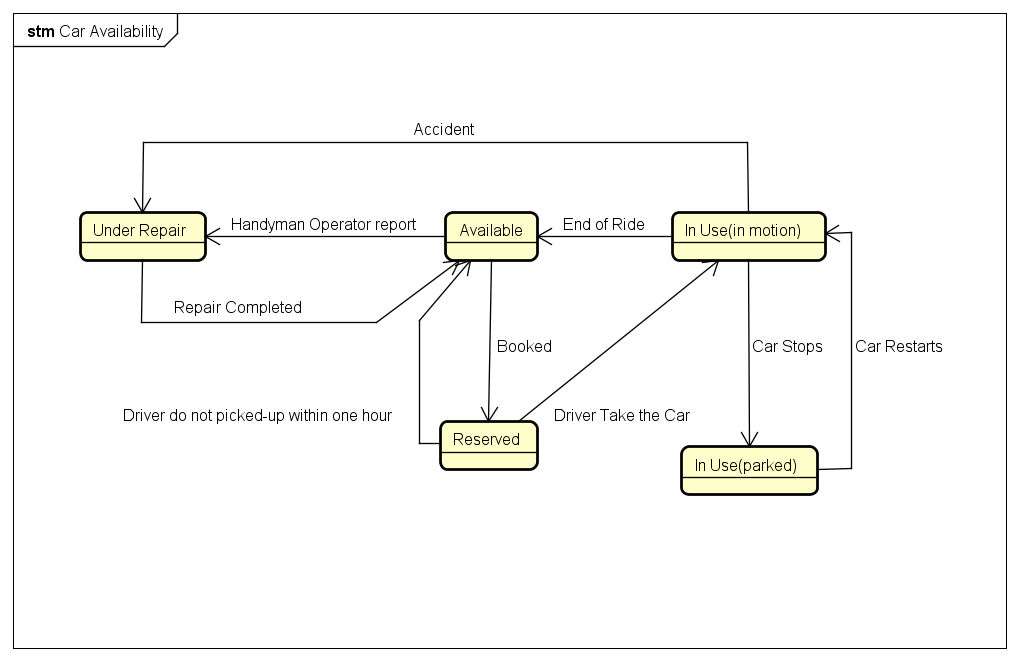
\includegraphics[keepaspectratio=true,scale=0.55]{img/state-machine-car-availability}}
			\end{minipage}	
			
			\vspace*{1cm}
		
		\subsection{Non Functional Requirements}
			\subsubsection{Performance Requirements}
			To ensure an high level of usability of the service it is important to calibrate the server resources. The objective is to avoid a deadlock due to the overload in situations of heavy loads.
			\subsubsection{Availability \& Reliability}
			The system must guarantee an availability of 98\%. The application will be hosted by multiple redundant servers to prevent service failures due to hardware faults. All servers will be equipped with an autonomous power supply backup system.
			
			\subsubsection{Security}
			All the communications between servers and clients must be protected by strong encryption using the SSL protocol. Users' passwords must not be stored in plain text in the database. The application must generate a snapshot of the last 10 days system's state.
			
			\subsubsection{Maintainability}
			When finished the software will not require any particular update except for security fix and the maintenance for APIs offered by the system. The code should be well documented to help developers to understand and edit it quickly.
			
		\pagebreak

		%---------------------------		ALLOY			-----------------------------
		\subsection{Alloy}
		\lstinputlisting[language=alloy,basicstyle=\normalsize]{alloy/alloy.als}
		\pagebreak
		\includegraphics[angle=90,keepaspectratio=true,scale=0.26]{"img/alloy"}
		
		
	\pagebreak
	
	
	
	%---------------------------		APPENDIX		-----------------------------
	
	\section{Appendix}
	
	\subsection{Software and tools used} 
	
	\begin{itemize}
		\item TeXstudio v2.11.2 (http://www.texstudio.org/) to produce this document.
		\item Evolus Pencil v2.0.5 (http://pencil.evolus.vn/) to generate mockups.
		\item Astah Professional 7.1.0 (http://astah.net/) to create Use Cases Diagrams, Sequence Diagrams, Class Diagrams and State Machine Diagrams. 
		\item Alloy Analyzer 4.2 (http://alloy.mit.edu/alloy/) to verify the consistency of the model.
	\end{itemize}
	
	\subsection{Hours of work} The time spent to redact this document:
	\begin{itemize}
		\item Bresich Matteo: 63 hours.
	\end{itemize}
	
	\begin{center}
		\begin{tabular}{ | l | l |}
			\hline
			Days & Hours of work\\ \hline
			27/10/16 & 2h\\\hline
			28/10/16 & 5h 30' \\\hline
			31/10/16 & 5h \\\hline
			03/11/16 & 3h \\\hline
			05/11/16 & 5h 30' \\\hline
			07/11/16 & 6h 30' \\\hline
			08/11/16 & 7h \\\hline
			09/11/16 & 7h \\\hline
			10/11/16 & 6h 30' \\\hline
			11/11/16 & 5h\\\hline
			12/11/16 & 2h\\\hline
			13/11/16 & 8h\\\hline

		\end{tabular}
	\end{center}
	
\end{document}